\documentclass[12pt, letterpaper]{article}
\author{Копылов Иван Александрович}
\usepackage[T1,T2A]{fontenc}
\usepackage[utf8]{inputenc}
\usepackage[english, russian]{babel}
\usepackage{graphicx}
\usepackage{booktabs}
\usepackage{amssymb}
\usepackage{amsmath}
\usepackage{listings}
\usepackage{a4, marginfit}
\usepackage{multirow}
\graphicspath{{images/}}
\lstset{
basicstyle=\fontencoding{T1}\ttfamily\small,
breaklines=true,
columns=fullflexible,
keepspaces=true,
frame=single,
language=Python
}
\title{Градиентные методы многомерной минимизации и методы второго порядка}
\date{Москва 2026}
\begin{document}
\maketitle
Лабораторная работа №3 

Вариант 10

Копылов Иван Александрович, БИВТ-24-9\\

\includegraphics[width=2cm]{signature.jpg} \\
НИТУ МИСИС \\
Лычёв Андрей Владимирович

\newpage

\section{Цель работы}
Приобретение практических навыков для решения задач многомерной минимизации градиентными методами и методами второго порядка.

\section{Задача}
Требуется найти безусловный минимум функции многих переменных $y = f(x_1, \dots, x_n)$, 
то есть такую точку $x^* \in \mathbb{R}^n$, что 
$f(x^*) = \min\limits_{x \in \mathbb{R}^n} f(x)$.

Согласно варианту 10:
\begin{itemize}
\item \textbf{Для градиентных методов:} \\
$f(x_1, x_2) = x_1^2 + x_1 x_2 + x_2^2 - 3x_1 - 6x_2$
\item \textbf{Для методов второго порядка:} \\
$f(x_1, x_2) = 100(x_2 - x_1^3)^2 + x_2^2 + x_1^2$
\end{itemize}

\section{GenAI}
\textbf{Использованные инструменты GenAI:}
\begin{enumerate}
\item OpenAI --- GPT-5. Использовался для оформления отчёта по данным из программного кода и генерации шаблона LaTeX.
\item Ollama --- Gemma4. Использовалась для оформления некоторых графиков.
\end{enumerate}

\section{Графическое представление функций на заданных интервалах}
\begin{center}
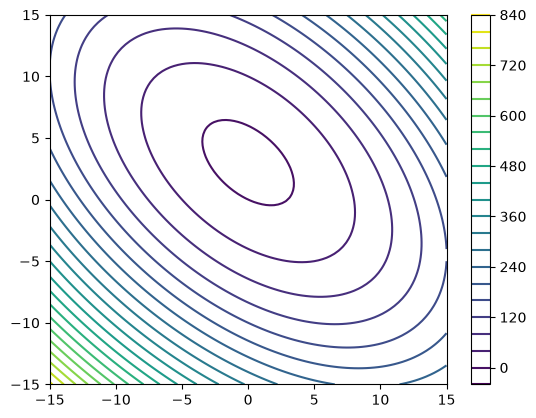
\includegraphics[width=0.8\textwidth]{grad_func.png} \\
\textit{Рис. 1. Контурный график функции для градиентных методов}
\end{center}
\begin{center}
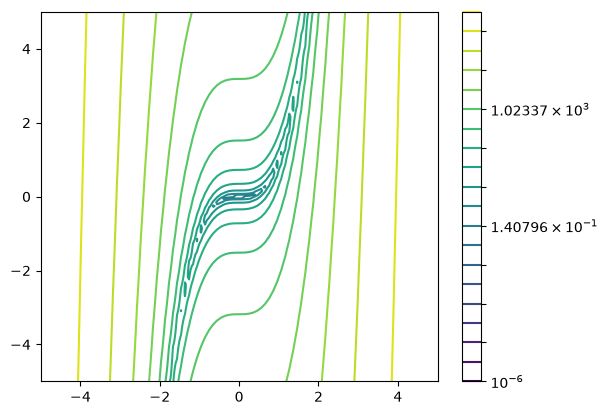
\includegraphics[width=0.8\textwidth]{sec_func.png} \\
\textit{Рис. 2. Контурный график функции для метода второго порядка}
\end{center}

\section{Аналитическое нахождение минимума}
\subsection*{Для градиентных методов}
Найдём частные производные и приравняем их к нулю:
\[
\frac{\partial f}{\partial x_1} = 2x_1 + x_2 - 3 = 0, \quad
\frac{\partial f}{\partial x_2} = x_1 + 2x_2 - 6 = 0.
\]
Решая систему уравнений, получаем:
\[
x_1 = 0, \quad x_2 = 3.
\]
Проверим достаточное условие экстремума с помощью матрицы Гесса:
\[
H = \begin{pmatrix}
2 & 1  \\
1 & 2
\end{pmatrix}.
\]
Так как $\Delta = 2 \cdot 2 - 1 \cdot 1 = 3 > 0$ и $f_{x_1 x_1} = 2 > 0$, матрица положительно определена, следовательно, точка $(0, 3)$ является точкой минимума.
Значение функции в точке минимума:
\[
f(0, 3) = 0^2 + 0 \cdot 3 + 3^2 - 3 \cdot 0 - 6 \cdot 3 = -9.
\]

\subsection*{Для метода второго порядка}
Найдём частные производные:
\[
\frac{\partial f}{\partial x_1} = -600x_1^2(x_2 - x_1^3) + 2x_1 = 0,
\]
\[
\frac{\partial f}{\partial x_2} = 200(x_2 - x_1^3) + 2x_2 = 0 \Rightarrow 202x_2 = 200x_1^3 \Rightarrow x_2 = \frac{100}{101}x_1^3.
\]
Подставим $x_2$ в первое уравнение:
\[
-600x_1^2\left(\frac{100}{101}x_1^3 - x_1^3\right) + 2x_1 = 0 \Rightarrow -\frac{600}{101}x_1^5 + 2x_1 = 0 \Rightarrow x_1\left(2 - \frac{600}{101}x_1^4\right) = 0.
\]
Единственным действительным корнем является $x_1 = 0$, откуда $x_2 = 0$.
Матрица Гесса в точке $(0, 0)$:
\[
H = \begin{pmatrix} 2 & 0 \\ 0 & 202 \end{pmatrix}.
\]
Матрица положительно определена, следовательно, точка $(0, 0)$ --- точка минимума.
Значение функции: $f(0, 0) = 0$.

\section{Листинг программы (градиентные методы)}
\begin{lstlisting}
import math
import matplotlib.pyplot as plt
from matplotlib.colors import LogNorm
import numpy as np

def f_base(x1, x2):
    ans = x1**2 + x1*x2 + x2**2 - 3*x1 - 6*x2
    return ans

def g_base(x1, x2):
    dx1 = 2*x1 + x2 - 3
    dx2 = 2*x2 + x1 - 6
    return dx1, dx2


# graph
x = np.linspace(-15, 15, 100)
y = np.linspace(-15, 15, 100)
X, Y = np.meshgrid(x, y)
Z = f_base(X, Y)

plt.contour(X, Y, Z, levels=20)
plt.colorbar()
plt.show()

# Gradient descend method with constant step
def method_1(eps, alpha = 0):
    iter_c = 0
    f_call_c = 0
    if alpha == 0:
        alpha = eps

    def f(x1, x2):
        nonlocal f_call_c
        f_call_c += 1
        return f_base(x1, x2)

    def g(x1, x2):
        nonlocal f_call_c
        f_call_c += 1
        return g_base(x1, x2)

    x1, x2 = 0, 0
    dx1, dx2 = g(x1, x2)
    run = [(x1, x2)]

    while math.sqrt(dx1**2 + dx2**2) > eps:
        iter_c += 1
        x1 = x1 - alpha * dx1
        x2 = x2 - alpha * dx2
        dx1, dx2 = g(x1, x2)

        run.append((x1, x2))

    return ((x1, x2), f(x1, x2), iter_c, f_call_c, run)

# Ravine method
def method_2(eps, alpha = 0, beta=0):
    iter_c = 0
    f_call_c = 0
    run = []

    if(alpha == 0):
        alpha = eps
        beta = 10 * alpha

    def f(x1, x2):
        nonlocal f_call_c
        f_call_c += 1
        return f_base(x1, x2)

    def g(x1, x2):
        nonlocal f_call_c
        f_call_c += 1
        return g_base(x1, x2)

    def grad_desc(x1, x2, dx1, dx2):
        nonlocal iter_c, run

        dx1, dx2 = g(x1, x2)

        while math.sqrt(dx1**2 + dx2**2) > eps:
            iter_c += 1

            x1 = x1 - alpha * dx1
            x2 = x2 - alpha * dx2
            run.append((x1, x2))
            # if abs(run[-1][1] - run[-2][1]) > 1: 
            #     print(run[-2][0], run[-2][1], run[-1][0], run[-1][1]) 
            
            dx1, dx2 = g(x1, x2)

        return x1, x2, dx1, dx2

    x1, x2 = 0, 0
    dx1, dx2 = g(x1, x2)

    y1 = x1 - alpha * dx1
    y2 = x2 - alpha * dx2
    dy1, dy2 = g(y1, y2)

    trick = [(x1, x2), (y1, y2)]

    x1, x2, dx1, dx2 = grad_desc(x1, x2, dx1, dx2)
    run = trick
    y1, y2, dy1, dy2 = grad_desc(y1, y2, dy1, dy2)

    while math.sqrt(dy1**2 + dy2**2) > eps:
        iter_c += 1

        d1 = y1 - x1
        d2 = y2 - x2
        if abs(d1) > 1: print(d1)
        if abs(d2) > 1: print(d2)

        z1 = y1 + beta * d1
        z2 = y2 + beta * d2
        dz1, dz2 = g(z1, z2)
        run.append((z1, z2))

        x1, x2, dx1, dx2 = y1, y2, dy1, dy2
        y1, y2, dy1, dy2 = grad_desc(z1, z2, dz1, dz2)
            
    return ((y1, y2), f(y1, y2), iter_c, f_call_c, run)

runs = []
mt_runs = []
for eps in (1e-2, 1e-4, 1e-6):

    ((x, y), f, iter_c, f_call_c, run) = method_1(eps, 0.01)
    print(eps, f_call_c, iter_c, (x, y), f)
    mt_runs.append(run)

runs.append(mt_runs)
    
print()
mt_runs = []
for eps in (1e-2, 1e-4, 1e-6):
    ((x, y), f, iter_c, f_call_c, run) = method_2(eps, 0.01)
    print(eps, f_call_c, iter_c, (x, y), f)
    mt_runs.append(run)
runs.append(mt_runs)

fig, axes = plt.subplots(2, 3, figsize=(18, 12))

method_names = ['Gradient descend method', 'ravine method'] 
epsilon_values = [0.01, 0.0001, 0.000001]
clrs = ['red', 'green', 'blue']

for row_idx in range(2):  # Different methods
    for col_idx in range(3):  # Different epsilons
        ax = axes[row_idx, col_idx]
        
        # Grid for this subplot
        x = np.linspace(-1, 1, 200)
        y = np.linspace(-1, 5, 200)
        X, Y = np.meshgrid(x, y)
        
        Z = f_base(X, Y)
        
        # Shift because log scale requires positive values
        Z_log = Z - Z.min() + 1e-6
        
        levels = np.logspace(
            np.log10(Z_log.min()),
            np.log10(Z_log.max()),
            20
        )
        
        # Contour plot
        ax.contour(
            X, Y, Z_log,
            levels=levels,
            norm=LogNorm()
        )
        
        # Get the trajectory for this method and epsilon
        print(row_idx, col_idx)
        run = runs[row_idx][col_idx]
        
        # Trajectory
        x_path = [point[0] for point in run]
        y_path = [point[1] for point in run]
        
        ax.plot(
            x_path,
            y_path,
            color=clrs[col_idx],
            linewidth=2,
            label=f'e={epsilon_values[col_idx]}'
        )
        
        ax.set_xlim(-1, 1)
        ax.set_ylim(-1, 5)
        
        ax.set_xlabel("x1")
        ax.set_ylabel("x2")
        
        # Set title based on position
        if row_idx == 0:
            ax.set_title(f"e = {epsilon_values[col_idx]}")
        else:
            ax.set_title("")
        
        # Add method label on the left
        if col_idx == 0:
            ax.text(-0.05, 0.5, method_names[row_idx], 
                   transform=ax.transAxes, rotation=90, 
                   verticalalignment='center', fontsize=12, fontweight='bold')
        
        ax.grid(True)
        ax.legend(loc='upper right', fontsize=8)

plt.suptitle('Optimization Trajectories: Methods vs Epsilon Values', fontsize=14, fontweight='bold', y=1.02)
plt.tight_layout()
plt.show()
\end{lstlisting}

\section{Листинг программы (методы 2 порядка)}
\begin{lstlisting}
    # %%
import math
import matplotlib.pyplot as plt
import numpy as np
from matplotlib.colors import LogNorm


# %%
def f_base(x1, x2):
    ans = 100*(x2 - x1**3)**2 + x2**2 + x1**2
    return ans

def g_base(x1, x2):
    dx1 = 2*x1 + 600*x1**5 - 600*x2*x1**2
    dx2 = 202*x2 - 200*x1**3
    return (dx1, dx2)

def H_base(x1, x2):
    x1x1 = 2 + 3000*x1**4 - 1200*x2*x1
    x1x2 = -600*x1**2
    x2x1 = -600*x1**2
    x2x2 = 202
    return [[x1x1, x1x2], [x2x1, x2x2]]

# %%

x = np.linspace(-5, 5, 100)
y = np.linspace(-5, 5, 100)
X, Y = np.meshgrid(x, y)
Z = f_base(X, Y)

Z_log = Z - Z.min() + 1e-6

levels = np.logspace(np.log10(Z_log.min()), np.log10(Z_log.max()), 20)

plt.contour(X, Y, Z_log, levels=levels, norm=LogNorm())
plt.colorbar()
plt.show()

# %%
# Newton method
def method_1(eps, x, y):
    iter_c = 0
    f_call_c = 0

    def f(x1, x2):
        nonlocal f_call_c
        f_call_c += 1
        return f_base(x1, x2)

    def d(x1, x2):
        nonlocal f_call_c
        f_call_c += 1
        return g_base(x1, x2)

    def H(x1, x2):
        nonlocal f_call_c
        f_call_c += 1
        return H_base(x1, x2)

    x1, x2 = x, y
    run = [(x1, x2)]

    while True:
        grad = d(x1, x2)
        hess = H(x1, x2)

        delta = np.linalg.solve(
            np.array(hess),
            -np.array(grad)
        )

        x1_new = x1 + delta[0]
        x2_new = x2 + delta[1]

        iter_c += 1

        if math.sqrt((x1_new - x1)**2 + (x2_new - x2)**2) < eps:
            x1, x2 = x1_new, x2_new
            break

        x1 = x1_new
        x2 = x2_new
        run.append((x1, x2))
    
    return ((x1, x2), f(x1, x2), iter_c, f_call_c, run)

# %%
runs = []
for (x, y) in ((1, 1), (10, 0), (-5, -3)):
    for eps in (1e-2, 1e-4, 1e-6): 
        ((x_m, y_m), f, iter_c, f_call_c, run) = method_1(eps, x, y)
        print(eps, iter_c, f_call_c, (x_m, y_m), f)

        if eps == 1e-6:
            runs.append(run)
    print()


# %%
fig, axes = plt.subplots(1, 3, figsize=(18, 6))

ranges = [
    (-2, 2, -2, 2),
    (-1, 11, -1, 11),
    (-6, 2, -6, 2)
]

for i, (ax, run, (x_min, x_max, y_min, y_max)) in enumerate(
    zip(axes, runs, ranges)
):
    x = np.linspace(x_min, x_max, 200)
    y = np.linspace(y_min, y_max, 200)
    X, Y = np.meshgrid(x, y)

    Z = f_base(X, Y)

    Z_log = Z - Z.min() + 1e-6

    levels = np.logspace(
        np.log10(Z_log.min()),
        np.log10(Z_log.max()),
        20
    )

    ax.contour(
        X, Y, Z_log,
        levels=levels,
        norm=LogNorm()
    )

    x_path = [point[0] for point in run]
    y_path = [point[1] for point in run]

    ax.plot(
        x_path,
        y_path,
        marker='o',
        color='red'
    )

    ax.set_xlim(x_min, x_max)
    ax.set_ylim(y_min, y_max)

    ax.set_xlabel("x1")
    ax.set_ylabel("x2")
    ax.set_title(f"Run {i + 1}")
    ax.grid(True)

plt.tight_layout()
plt.show()
\end{lstlisting}

\section{Результаты вычислений}
\subsection*{Градиентные методы}

\begin{center}
\small
\resizebox{\textwidth}{!}{%
\begin{tabular}{c c c c c}
\toprule
\multirow{2}{*}{$\varepsilon$} & \multicolumn{4}{c}{Метод 1 (Градиентный спуск)} \\
\cmidrule(lr){2-5}
& Вычисл. & Итер. & Решение & $f(x^*)$ \\
\midrule
$10^{-2}$ & 536 & 534 & $(0.0070028874, 2.9929968536)$ & $-8.9999509578$ \\
$10^{-4}$ & 994 & 992 & $(7.0178535192\cdot10^{-5}, 2.9999298215)$ & $-8.9999999950$ \\
$10^{-6}$ & 1452 & 1450 & $(7.0327215955\cdot10^{-7}, 2.9999992967)$ & $-8.9999999999$ \\
\bottomrule
\end{tabular}%
}
\end{center}

\begin{center}
\small
\resizebox{\textwidth}{!}{%
\begin{tabular}{c c c c c}
\toprule
\multirow{2}{*}{$\varepsilon$} & \multicolumn{4}{c}{Метод 3 (Овражный метод)} \\
\cmidrule(lr){2-5}
& Вычисл. & Итер. & Решение & $f(x^*)$ \\
\midrule
$10^{-2}$ & 1072 & 1067 & $(0.0070028874, 2.9929968536)$ & $-8.9999509578$ \\
$10^{-4}$ & 1988 & 1983 & $(7.0178535192\cdot10^{-5}, 2.9999298215)$ & $-8.9999999951$ \\
$10^{-6}$ & 2904 & 2899 & $(7.0327215955\cdot10^{-7}, 2.9999992967)$ & $-8.9999999999$ \\
\bottomrule
\end{tabular}%
}
\end{center}

\subsection*{Метод второго порядка (Ньютона)}
\begin{center}
\small
\resizebox{\textwidth}{!}{%
\begin{tabular}{c c c c c}
\toprule
Начальная точка & Погрешность & Число итераций & Оптимальное решение & Оптимальное значение \\
\midrule
$(1, 1)$ & $10^{-2}$ & 8 & $(2.7311660895\cdot10^{-14}, -4.4202414352\cdot10^{-17})$ & $7.4612416002\cdot10^{-28}$ \\
$(1, 1)$ & $10^{-4}$ & 8 & $(2.7311660895\cdot10^{-14}, -4.4202414352\cdot10^{-17})$ & $7.4612416002\cdot10^{-28}$ \\
$(1, 1)$ & $10^{-6}$ & 9 & $(0, 0)$ & $0$ \\

$(10, 0)$ & $10^{-2}$ & 29 & $(8.8978326863\cdot10^{-7}, -1.0579454127\cdot10^{-9})$ & $7.9182730924\cdot10^{-13}$ \\
$(10, 0)$ & $10^{-4}$ & 30 & $(5.0260817508\cdot10^{-19}, -1.3949586258\cdot10^{-18})$ & $1.9678948131\cdot10^{-34}$ \\
$(10, 0)$ & $10^{-6}$ & 30 & $(5.0260817508\cdot10^{-19}, -1.3949586258\cdot10^{-18})$ & $1.9678948131\cdot10^{-34}$ \\

$(-5, -3)$ & $10^{-2}$ & 23 & $(-6.9007481376\cdot10^{-7}, 8.2057799011\cdot10^{-10})$ & $4.7627125676\cdot10^{-13}$ \\
$(-5, -3)$ & $10^{-4}$ & 24 & $(-2.3441636815\cdot10^{-19}, 6.5072458313\cdot10^{-19})$ & $4.2822641825\cdot10^{-35}$ \\
$(-5, -3)$ & $10^{-6}$ & 24 & $(-2.3441636815\cdot10^{-19}, 6.5072458313\cdot10^{-19})$ & $4.2822641825\cdot10^{-35}$ \\
\bottomrule
\end{tabular}%
}
\end{center}

\section{Графическое представление траекторий}
\begin{center}
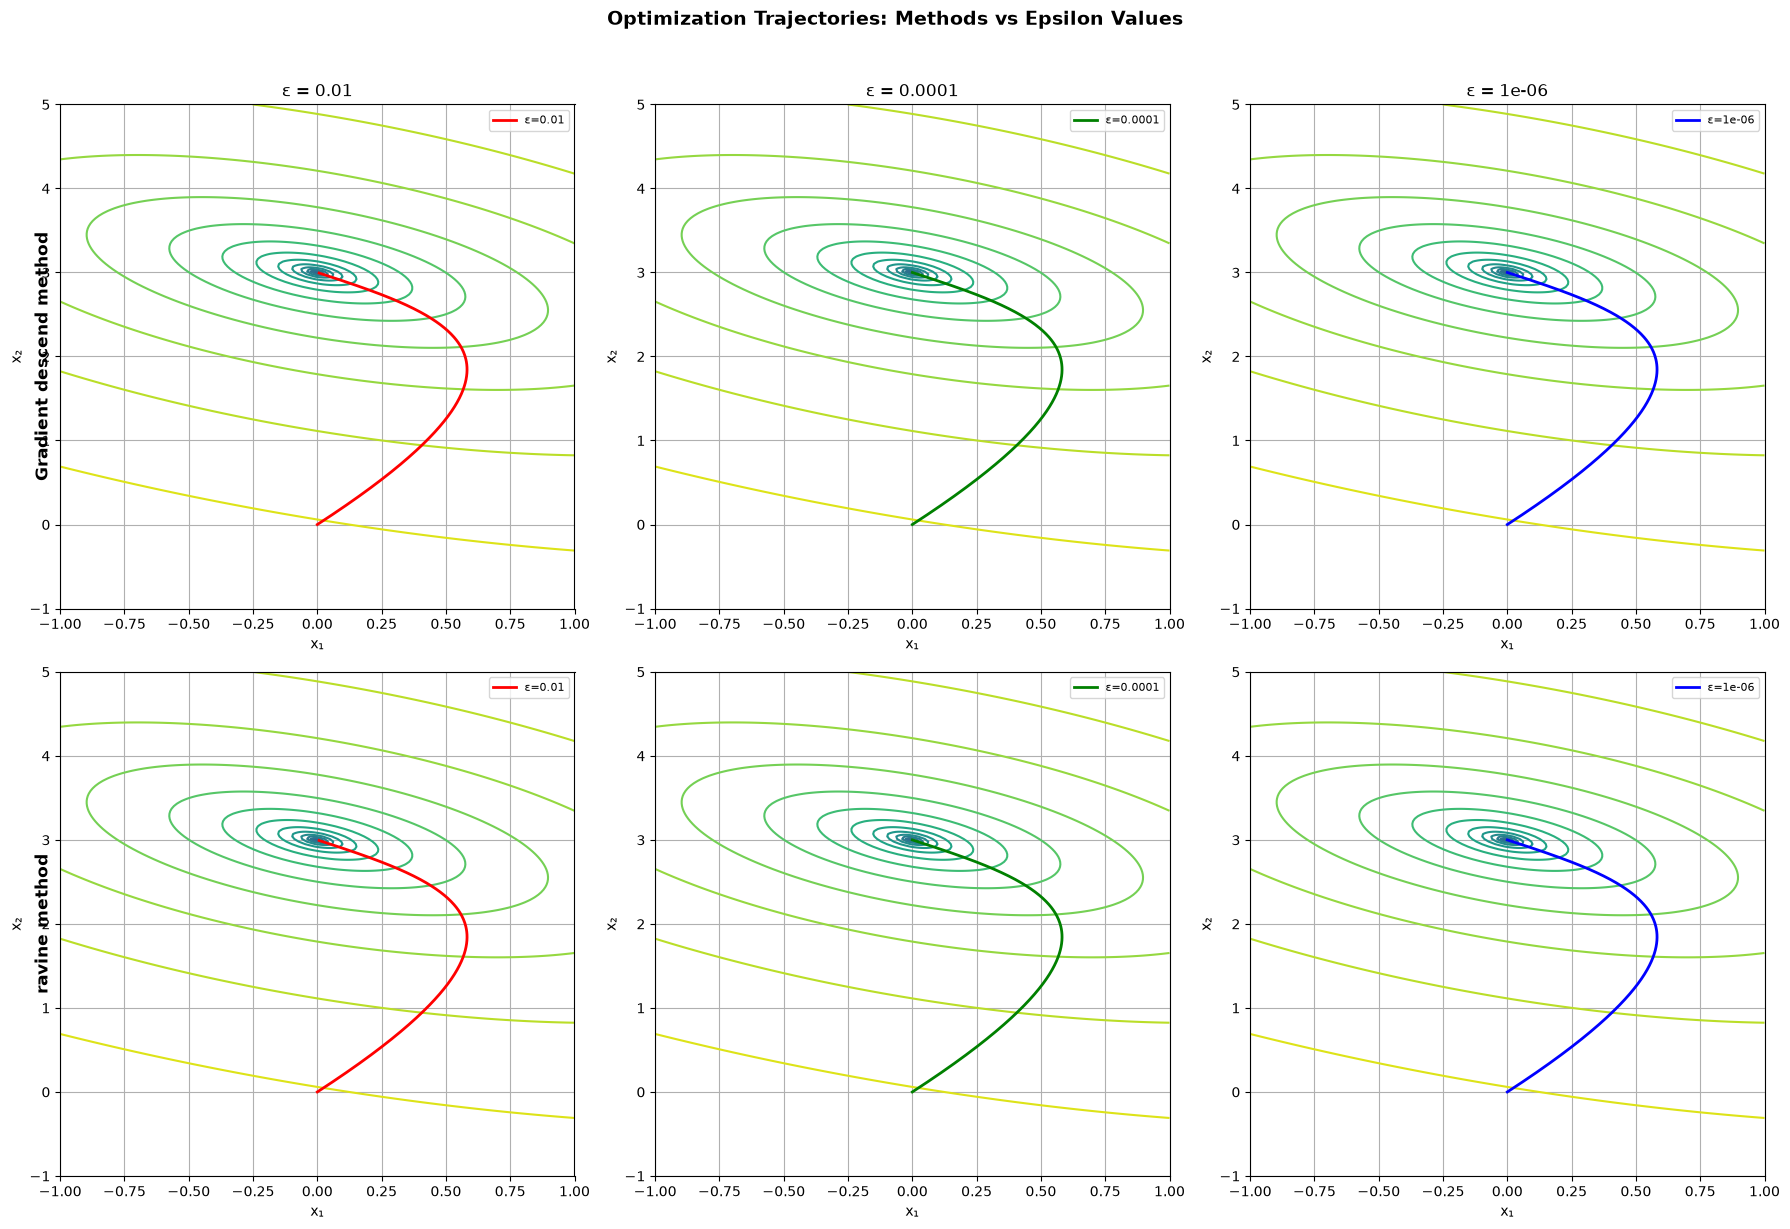
\includegraphics[width=0.8\textwidth]{grad_traj.png} \\
\textit{Рис. 3. Траектории сходимости градиентных методов}
\end{center}
\begin{center}
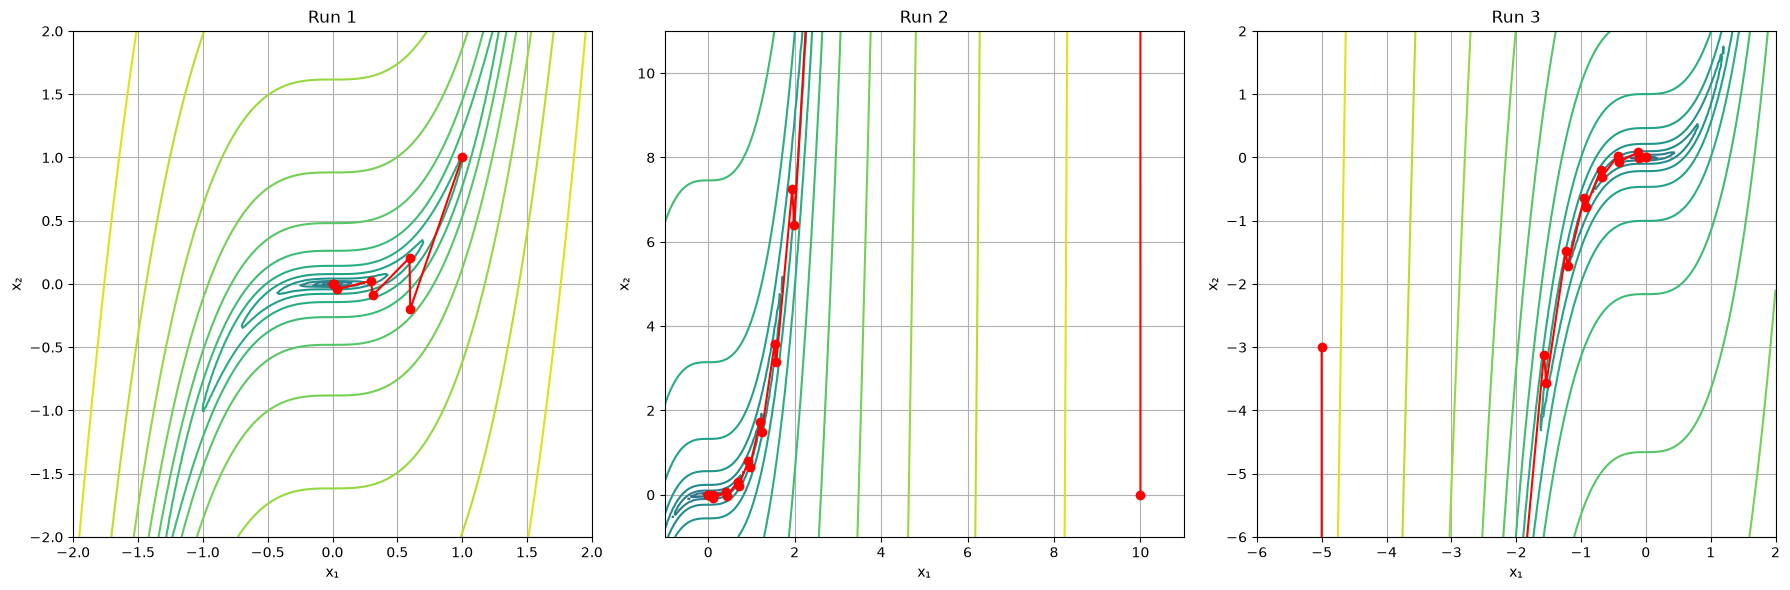
\includegraphics[width=0.8\textwidth]{sec_traj.png} \\
\textit{Рис. 4. Траектории сходимости метода Ньютона для различных начальных точек}
\end{center}

\section{Сравнительная характеристика методов}
\textbf{Градиентные методы:}
Для заданной квадратичной функции метод градиентного спуска с постоянным шагом (Метод 1) показал себя эффективнее овражного метода (Метод 3) по количеству вычислений. Овражный метод требует дополнительных вычислений градиента на каждом шаге (для проверки условия остановки и корректировки направления), что при простой топологии функции (отсутствие глубоких оврагов) приводит к избыточному числу вызовов функции (примерно в 2 раза больше, чем у простого градиентного спуска). Оба метода успешно сходятся к аналитическому минимуму $(0, 3)$ с заданной точностью.

\textbf{Метод второго порядка:}
Метод Ньютона продемонстрировал выдающуюся эффективность. Благодаря использованию информации о втором порядке (матрицы Гесса), метод обладает квадратичной скоростью сходимости. Алгоритм сошелся к глобальному минимуму $(0, 0)$ за минимальное число итераций (от 8 до 30) для всех трех выбранных начальных точек, достигнув машинной точности ($\approx 10^{-19}$ по координатам). Это делает метод Ньютона предпочтительным для гладких функций с хорошо вычисляемой и невырожденной матрицей Гесса, несмотря на высокую стоимость вычисления самой матрицы Гесса на каждой итерации.

\section{Выводы}
В ходе лабораторной работы были изучены и реализованы градиентные методы и методы второго порядка для многомерной минимизации.

Аналитически найдены глобальные минимумы для обеих функций: $(0, 3)$ для первой и $(0, 0)$ для второй.

Экспериментально подтверждено, что для гладких квадратичных функций простой градиентный спуск может быть более экономичным по числу вычислений функции, чем овражный метод, который лучше проявляет себя на функциях с выраженной овражной структурой.

Метод Ньютона показал высочайшую скорость сходимости, достигая машинного нуля за считанные итерации независимо от начального приближения (в области притяжения минимума), что подтверждает его высокую эффективность для задач с хорошо обусловленной матрицей Гесса.
\end{document}